Возьмем из аксиоматики второй закон Ньютона и выберем какую-то параметризацию системы, которая хорошо описывает все ее точки. Эта параметризация есть криволинейные координаты. Введем понятие \textbf{обобщенных} координат --- это локально невырожденная параметризация конфигурационного многообразия механической системы, где \textbf{конфигурационное многообразие} --- множество всех точек, в которые теоретически может попасть система.\\

Понятия, описанные ниже, в дальнейшем будут изучены более подробно.\\

Найдем проекции второго закона Ньютона на направления локального базиса:
\[
m \cdot \dfrac{1}{h_k}\left[ \dfrac{d}{d t} \left( \dfrac{\partial \dfrac{v^2}{2}}{\partial \dot{q_k}}\right) - \dfrac{\partial \dfrac{v^2}{2}}{\partial q_k}\right] = \vec{F} \cdot \dfrac{\partial \vec{r}}{\partial q_k}
\]
Внесем массу m под дифференциалы и получим \textbf{кинетическую энергию} $T = \dfrac{mv^2}{2}$.\\

Пусть $Q_k = \vec{F} \dfrac{\partial \vec{r}}{\partial q_k}$ --- k-ая компонента \textbf{вектора обобщенных сил}. Также, введем \textbf{элементарную работу} силы F:
\[
\delta A = \vec{F} d \vec{r}
\]
Понятно, что
\[
\delta A = \vec{F} \dfrac{\partial \vec{r}}{\partial q_k} d q = Q dq
\]

\hypertarget{def_potential_force}{}
\begin{definition}
    

    Сила $\vec{F}(\vec{r},~ t)$ называется \textbf{потенциальной}, если существует такая скалярная функция П$(\vec{r},~ t)$, называемая \textbf{потенциальной энергией}, что
    \[
    \vec{F} = -\dfrac{\partial \text{П}(\vec{r},~ t)}{\partial \vec{r}} \tab \text{или} \tab \vec{Q} = \dfrac{\partial \text{П}(\vec{q},~ t)}{\partial \vec{q}}
    \]
    При этом сила F(П) является \textbf{консервативной} тогда и только тогда, когда П не зависит от времени t.
\end{definition}

Подставив это в проекции второго закона Ньютона, для потенциального Q получим
\[
\dfrac{d}{d t} \dfrac{\partial T}{\partial \dot{q}} - \dfrac{\partial T}{\partial q} = - \dfrac{\partial\text{П}}{\partial q}
\]
А введя функцию Лагранжа (правильно сделаем это позже) L = T - П, получим \textbf{Уравнение Лагранжа второго рода} (оно же --- оператор Эйлера).\\

\begin{frame}{Фан факт}
    Можно построить аксиоматику не через законы Ньютона, а через принцип наименьшего\\ действия: возьмем в качестве функционала
    \[
    W = \int\limits_{t_0}^t L (q, \dot{q}, t) d t
    \]
    Он нужен для оптимизации траектории, например определяет траекторию тела, летящего по параболе. Но на самом деле это не оптимум (для него нужно дополнительное условие), а стационарная точка.\\
\end{frame}




\begin{example}[Осциллятор]
\tab\\
    \begin{figure}[!h]
    	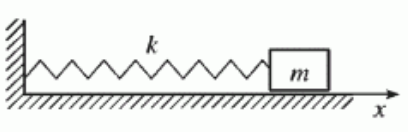
\includegraphics[width=0.3\linewidth]{images/лекция_2_2.png}
    \end{figure}
    \tab\\
    По второму закону Ньютона
    \[
    m\ddot{x} = -kx
    \]
    Найдем кинетическую и потенциальную энергии
    \[
    T = \dfrac{m\dot{x}^2}{2}, \tab \text{П} = \dfrac{kx^2}{2}
    \]
    Тогда лагранжиан
    \[
    L = \dfrac{m\dot{x}^2}{2} - \dfrac{kx^2}{2}
    \]
    Подставив его в опреатор Эйлера, получим все тот же второй закон Ньютона $m\ddot{x} = -kx$.

\end{example}


\subsection{Кинематика твердого тела}
\textbf{Твердое тело} --- множество точек, расстояние между которыми не меняется, т.е. $\forall i,~j \hookrightarrow \vec{r_i}\cdot \vec{r_j} = const$.\\

Введем систему координат, жестко привязанную к телу, для описания скоростей и ускорений.\\

\begin{wrapfigure}{l}{0.5\textwidth}
	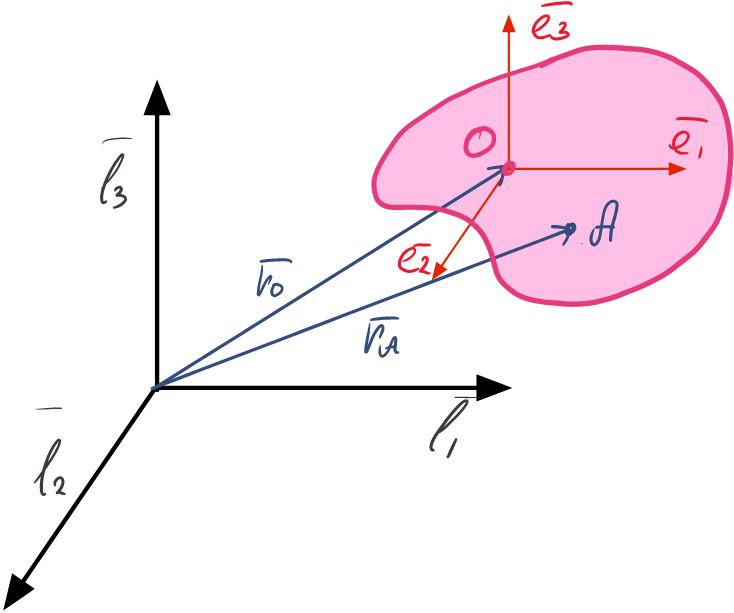
\includegraphics[width=0.8\linewidth]{images/лекция_2_4.jpeg}
\end{wrapfigure}

Пусть имеется неподвижная прямоугольная декартова система координат, в которой движется произвольное твердое тело с привязанной к нему другой системой координат (точка О --- начало отсчета в ней). Выберем в теле некоторую точку А. Точки О и А задаются в неподвижной системе соответственно радиус-векторами $\vec{r_O}$ и $\vec{r_A}$.\\

Тогда в неподвижной системе отсчета:
\[
\vec{r_A} = \vec{r_O} + \vec{OA}
\]
\[
\dot{\vec{r_A}} = \dot{\vec{r_O}} + \dot{\vec{OA}} \tab \Longrightarrow \tab \vec{v_A} = \vec{v_O} + \dot{\vec{OA}}
\]

Без ограничения общности можем считать, что О совпадает с началом координат неподвижного базиса.\\

\begin{wrapfigure}{r}{0.5\textwidth}
	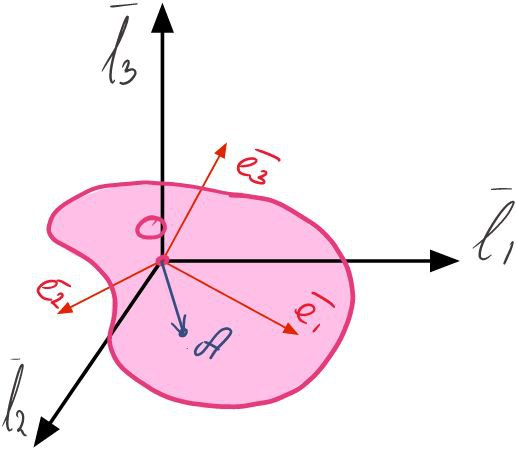
\includegraphics[width=0.7\linewidth]{images/лекция_2_5.jpeg}
\end{wrapfigure}

Тогда вектор $e_k$ задается следующим образом:
\[
\vec{e_k} = \begin{pmatrix}
    \cos{\angle \vec{l_1}\vec{e_k}}\\
    \cos{\angle \vec{l_2}\vec{e_k}}\\
    \cos{\angle \vec{l_3}\vec{e_k}}\\
\end{pmatrix}
\]

Пусть $\vec{r}_{OA}^l$ --- разложение по базису l, $\vec{r}_{OA}^e$ --- разложение по базису e. Тогда (из курса линейной алгебры):
\[
\vec{r}_{OA}^l = U \cdot \vec{r}_{OA}^e,
\]
где $U = [\vec{e_1}, \vec{e_2}, \vec{e_3}]$ --- матрица перехода (матрица направляющих косинусов). Понятно, что $\vec{e_i} \cdot \vec{e_j} = \delta_{ij}$, где $\delta_{ij}$ --- символ Кронекера, значит, в матрице 3 независимых параметра. Также из курса линейной алгебры известно, что 

\[
U \cdot U^T = U^T \cdot U = E
\]
\[
\dot{U} \cdot U^T + U\cdot \dot{U} ^T = 0
\]
\[
(\dot{U} \cdot U^T)^T = - \dot{U} U^T = \Omega,
\]
где $\Omega = \begin{pmatrix}
    0 & -\omega_z & \omega_y\\
    \omega_z & 0 & -\omega_x\\
    -\omega_y & \omega_x & 0\\
\end{pmatrix}$. Тогда
\[
\dot{\vec{r}}_{OA}^l = \dot{U}{\vec{r}_{OA}^e} = \dot{U}U^T{\vec{r}_{OA}^l} = \Omega \vec{r}_{OA}^l
\]
Откуда получаем, что $\Omega\vec{r}_{OA}^l = \vec{\omega}\times \vec{r}_{OA}^l$, где вектор $\vec{\omega} = (\omega_x, \omega_y, \omega_z)^T$ называется \textbf{угловой скоростью} твердого тела. Также, мы доказали следующую теорему.\\

\begin{theorem}
    При произвольном движении твердого тела в любой фиксированный момент времени существует и единственнен вектор $\vec{\omega}$ такой, что скорости любых двух точек связаны соотношением
    \[
    \vec{v_A} = \vec{v_O} + \vec{\omega} \times \vec{OA}
    \]
    Это соотношение называется \textbf{формулой Эйлера} (или формулой распределения скоростей точек твердого тела).
\end{theorem}
\begin{corollary}
    \tab\\
    \begin{enumerate}
        \item Пусть $\vec{a}$ $\Longrightarrow$ $\dot{\vec{a}} = \dot{a}\dfrac{\vec{a}}{a} + \vec{\omega} \times \vec{a}$.
        \item Для любых двух точек О и А внутри твердого тела при домножении обеих частей формулы Эйлера на $\vec{OA}$ и на $\vec{\omega}$ получим \textbf{кинематические инварианты} твердого тела:
        \[
        \vec{v}_A \cdot \vec{OA} = \vec{v}_O \cdot \vec{OA}
        \]
        \[
        \vec{v}_A \cdot \vec{\omega} = \vec{v}_O \cdot \vec{\omega}
        \]
        \item Двух точек не хватит для определения угловой скорости.
        \item \underline{Кинематический винт}.
        Пусть известны $\vec{v_O}$ и $\vec{\omega}$. Возьмем формулу Эйлера и скалярно домножим на $\omega$: получим инвариант $\forall O,~A$
        \[
        \vec{v_O}\cdot \vec{\omega} = \vec{v_A}\cdot \vec{\omega}
        \]
        Значит, существует компонента скорости, коллинеарная $\vec{\omega}$ $\vec{v}_{||} = \dfrac{\vec{v_O}\vec{\omega}}{\omega}\cdot \dfrac{\vec{\omega}}{\omega}$.\\
        
        Найдем точку B такую, что $\vec{v_O} = \vec{v}_{||}$.\\
        Очевидно, что $\vec{v_B} = \vec{v_O} + \vec{\omega}\times \vec{OB}$, $\vec{v_B}~ || ~\vec{\omega}$.
        \[
        \vec{OB} = \begin{pmatrix}
            x - x_O\\y - y_O\\z-z_O\\
        \end{pmatrix} \Longrightarrow  \begin{pmatrix}
            \omega_x\\ \omega_y \\ \omega_z
        \end{pmatrix} \times \begin{pmatrix}
            x - x_O\\y - y_O\\z - z_O\\
        \end{pmatrix} = const \Longrightarrow \text{получили уравнение прямой}
        \]
        Найти ускорение кинематического винта = найти ось винта и скоростью поступательного движения.
        \item \underline{Формула Ривальса}, или распределение ускорений точек твердого тела.\\
        Продифференцируем формулу Эйлера:
        \[
        \vec{w_A} = \vec{w_O} + \vec{\varepsilon} \times \vec{OA} + \vec{\omega} \times (\vec{\omega} \times \vec{OA}),
        \]
        где $\vec{\varepsilon}$ --- \textbf{угловое ускорение}, $\vec{\varepsilon} \cdot \vec{OA}$ --- \textbf{вращательное ускорение}, $\vec{\omega} \times (\vec{\omega} \times \vec{OA})$ --- \textbf{осестремительное ускорение}.
        \item \underline{Плоскопараллельное движение}.\\
        Пусть скорости всех точек коллинеарны плоскости $\alpha$ (без ограничения общности считаем, что это $O_{xy}$). Тогда
        \[
        \begin{pmatrix}
            v_A^x\\v_A^y\\v_A^z\\
        \end{pmatrix} = \begin{pmatrix}
            v_O^x\\v_O^y\\v_O^z\\
        \end{pmatrix} + \begin{pmatrix}
            \omega_x\\ \omega_y \\ \omega_z
        \end{pmatrix} \times \begin{pmatrix}
            x_A - x_O\\y_A - y_O\\z_A - z_O\\
        \end{pmatrix} \Longrightarrow \vec{\omega} \perp \alpha
        \]
        Значит
        \[
        \vec{w_A} = \vec{w_O} + \vec{\varepsilon} \times \vec{OA} - \omega^2\vec{OA}
        \]
    \end{enumerate}
\end{corollary}